\section{Проектирование прототипа}
В этом разделе будут описаны некоторые этапы проектирования прототипа акустической камеры. В результате исследования теоретических материалов и проведения некоторых экспериментов была разработана структурная схема проектируемого устройства, которая показана на рисунке~\ref{fig:MainStructural}. Дальнейшее проектирование производилось в соответствии с данной схемой.

\begin{figure}[ht]
	\centering
	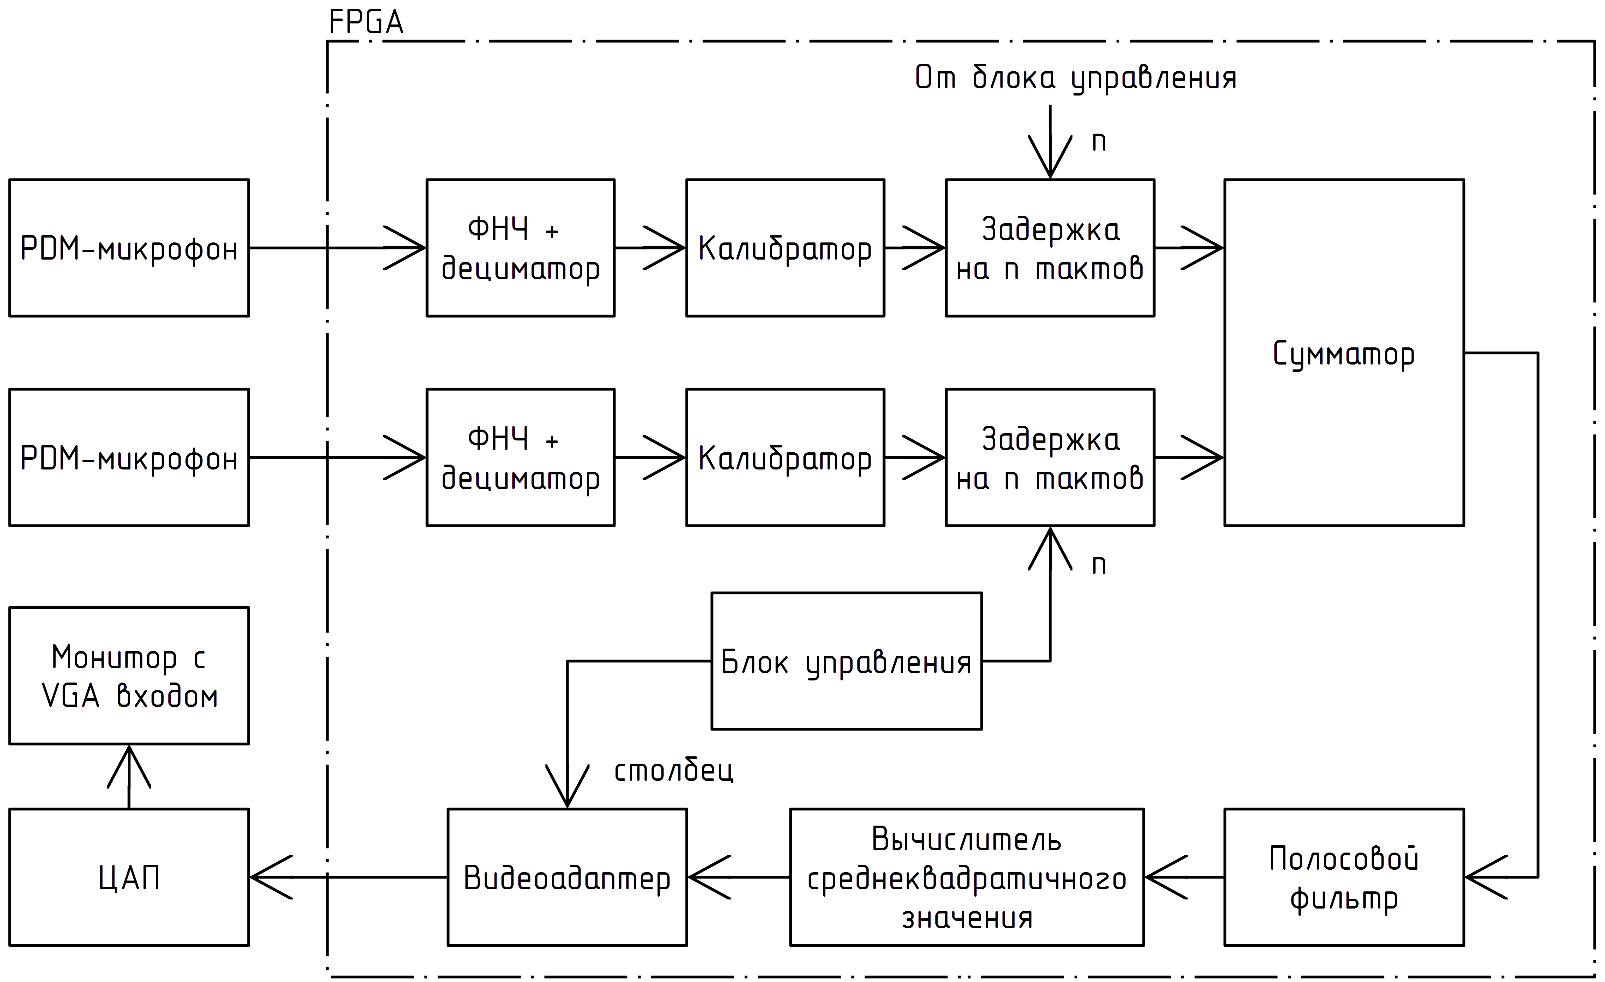
\includegraphics[scale=0.55]{MainStructural.png}  
	\caption{Структурная схема проектируемого устройства}
	\label{fig:MainStructural}
\end{figure}

% **************************************************
\subsection{Выбор параметров микрофонной решётки}
\label{section:MicArrayCalculations}
В виду сложности обработки данных с двумерной микрофонной решётки, в проекте решено применить одномерную микрофонную решётку. Единственным параметром характеризующим её конфигурацию является расстояние между микрофонами, которое необходимо рассчитать.

Уровень выходного сигнала полученного после суммирования отдельных сигналов со всех элементов линейной микрофонной решётки для определённой частоты можно вычислить по формуле~\cite{LabBookPages}:
\begin{equation}
	A = 20\lg{\left(\frac{1}{N}\sum_{i=0}^{N-1}e^{\frac{j2\pi{}fil\sin{\theta}}{c}}\right)}
\end{equation}
\begin{explanation}
	где &$A$& выходной сигнал, дБ; \\
	&$N$& количество датчиков микрофонной решётки; \\
	&$f$& частота входного сигнала, Гц; \\
	&$l$& расстояние между датчиками, м; \\
	&$c$& скорость звука, м/с; \\
	&$\theta$& угол падения звуковой волны на плоскость микрофонной решётки.
\end{explanation}

Построим зависимость уровня сигнала от $f$ и от $\theta$ при разных $N$ и $l$~\cite{LabBookPages} (см. рисунок~\ref{fig:BeamformerPatterns}). Для дальнейшего проектирования выберем решётку с параметрами $l = 0,04~\text{м}$ и $N = 15$. Выбор обусловлен следующими причинами:
\begin{itemize}
	\item Число микрофонов приемлемо для построения решётки в домашних условиях;
	\item Расстояние между микрофонами не слишком велико, следовательно общая длинна решётки останется приемлемой;
	\item Подавление сигнала вне диапазона чувствительности является вполне достаточным;
	\item Рабочий диапазон частот 3~--~6~кГц близок к спектру человеческого голоса;
\end{itemize}

Для удобства проектирования печатной платы, число микрофонов выберем равным 16.

\begin{figure}[ht]
	\centering
	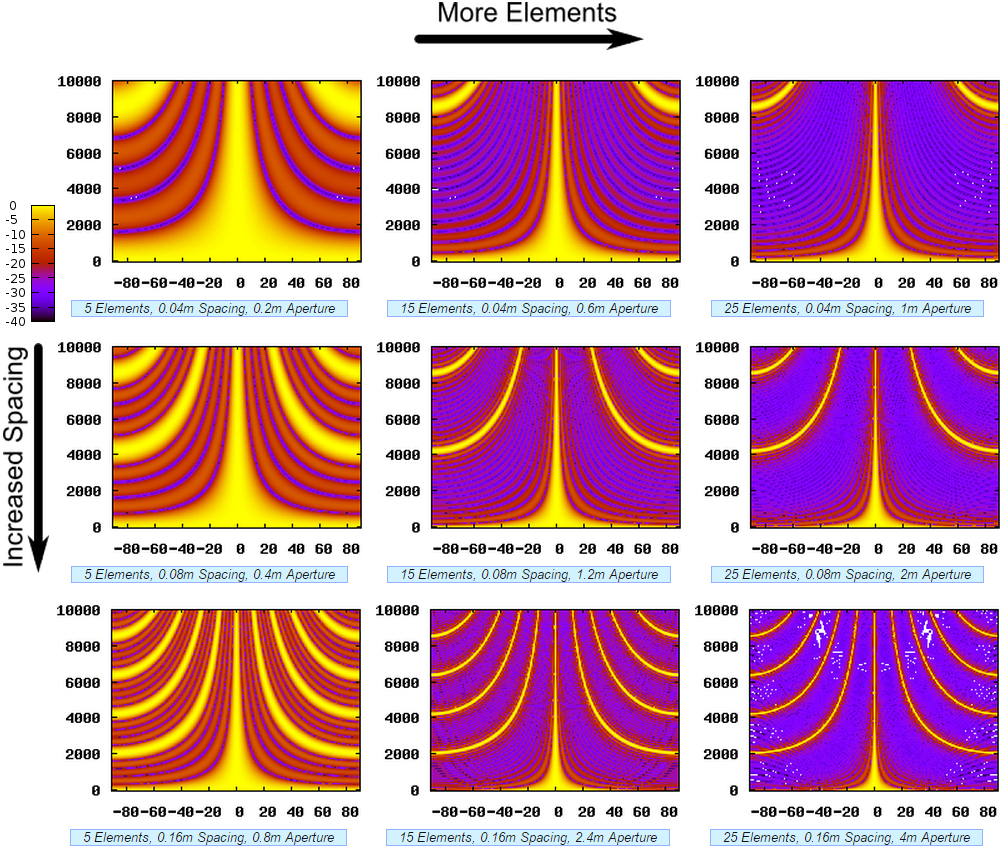
\includegraphics[scale=0.6]{BeamformerPatterns.png}  
	\caption{Зависимость уровня выходного сигнала бимформера от угла падения звуковой волны и от частоты сигнала при различном количестве датчиков и разном расстоянии между ними}
	\label{fig:BeamformerPatterns}
\end{figure}

% **************************************************
\subsection{Разработка печатных плат для микрофонной решётки}
\label{section:PcbBuilding}
Микрофоны применяемые в данном проекте выпускаются только в корпусах для поверхностного монтажа, поэтому для соединения каждого из них с блоком обработки данных, необходимо разработать и создать печатную плату. Учитывая, что микрофонная решётка состоит из 16-ти микрофонов, которые размещены на расстоянии 40 мм друг от друга, общая длинна платы равнялась бы не менее 0,6 метрам. Цельный кусок фольгированного текстолита такого размера достаточно трудно найти. Поэтому плата была разбита на 4 части по 160 мм каждая. Также была разработана плата-соединитель для подключения всех остальных плат к плате \boardname{}. 

В качестве программного обеспечения для проектирования платы была выбрана программа Sprint-Layout 6.0. Такой выбор обоснован простотой этой программы, а также простотой разрабатываемой платы, которая не требует каких либо особых возможностей от среды проектирования.

При проектировании рисунка печатной платы было соблюдено рассчитанное ранее расстояние между микрофонами в 40 мм. На края платы были добавлены контактные площадки для возможности её соединения с соседними платами. Стоит также отметить, что плата-соединитель, размещённая между двумя обычными платами увеличивает расстояние межу микрофонами. Поэтому, на плату были добавлены дополнительные контактные площадки на некотором расстоянии от края. Это позволит срезать часть платы со стороны прилегающей к плате-соединителю, не лишившись при этом контактных площадок.

В виду невозможности развести для данного проекта одностороннюю печатную плату без перемычек, шины данных микрофонов были выведены на специальные площадки и соединены с платой-соединителем с помощью проводов.

В результате разработки получилась печатная плата, показанная на рисунке~\ref{fig:Pcb4Mic}. Плата-соеденитель представлена на рисунке~\ref{fig:PcbConnector}

\begin{figure}[ht]
	\centering
	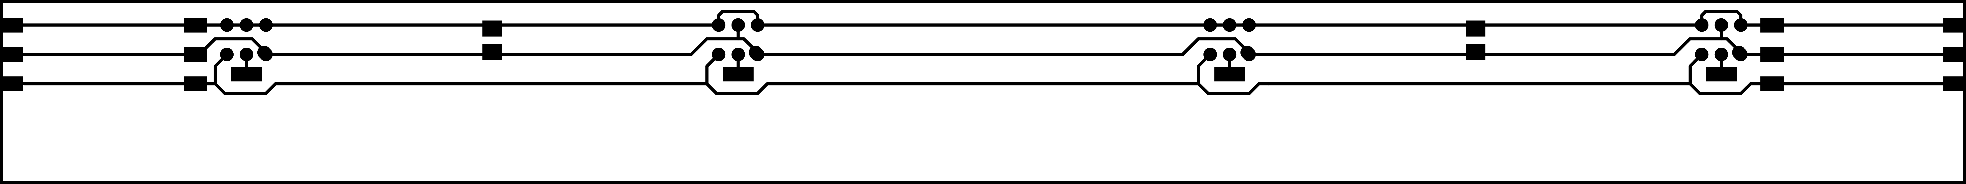
\includegraphics[scale=0.95]{Pcb4Mic.png}  
	\caption{Печатная плата для четырёх микрофонов}
	\label{fig:Pcb4Mic}
\end{figure}

\begin{figure}[ht]
	\centering
	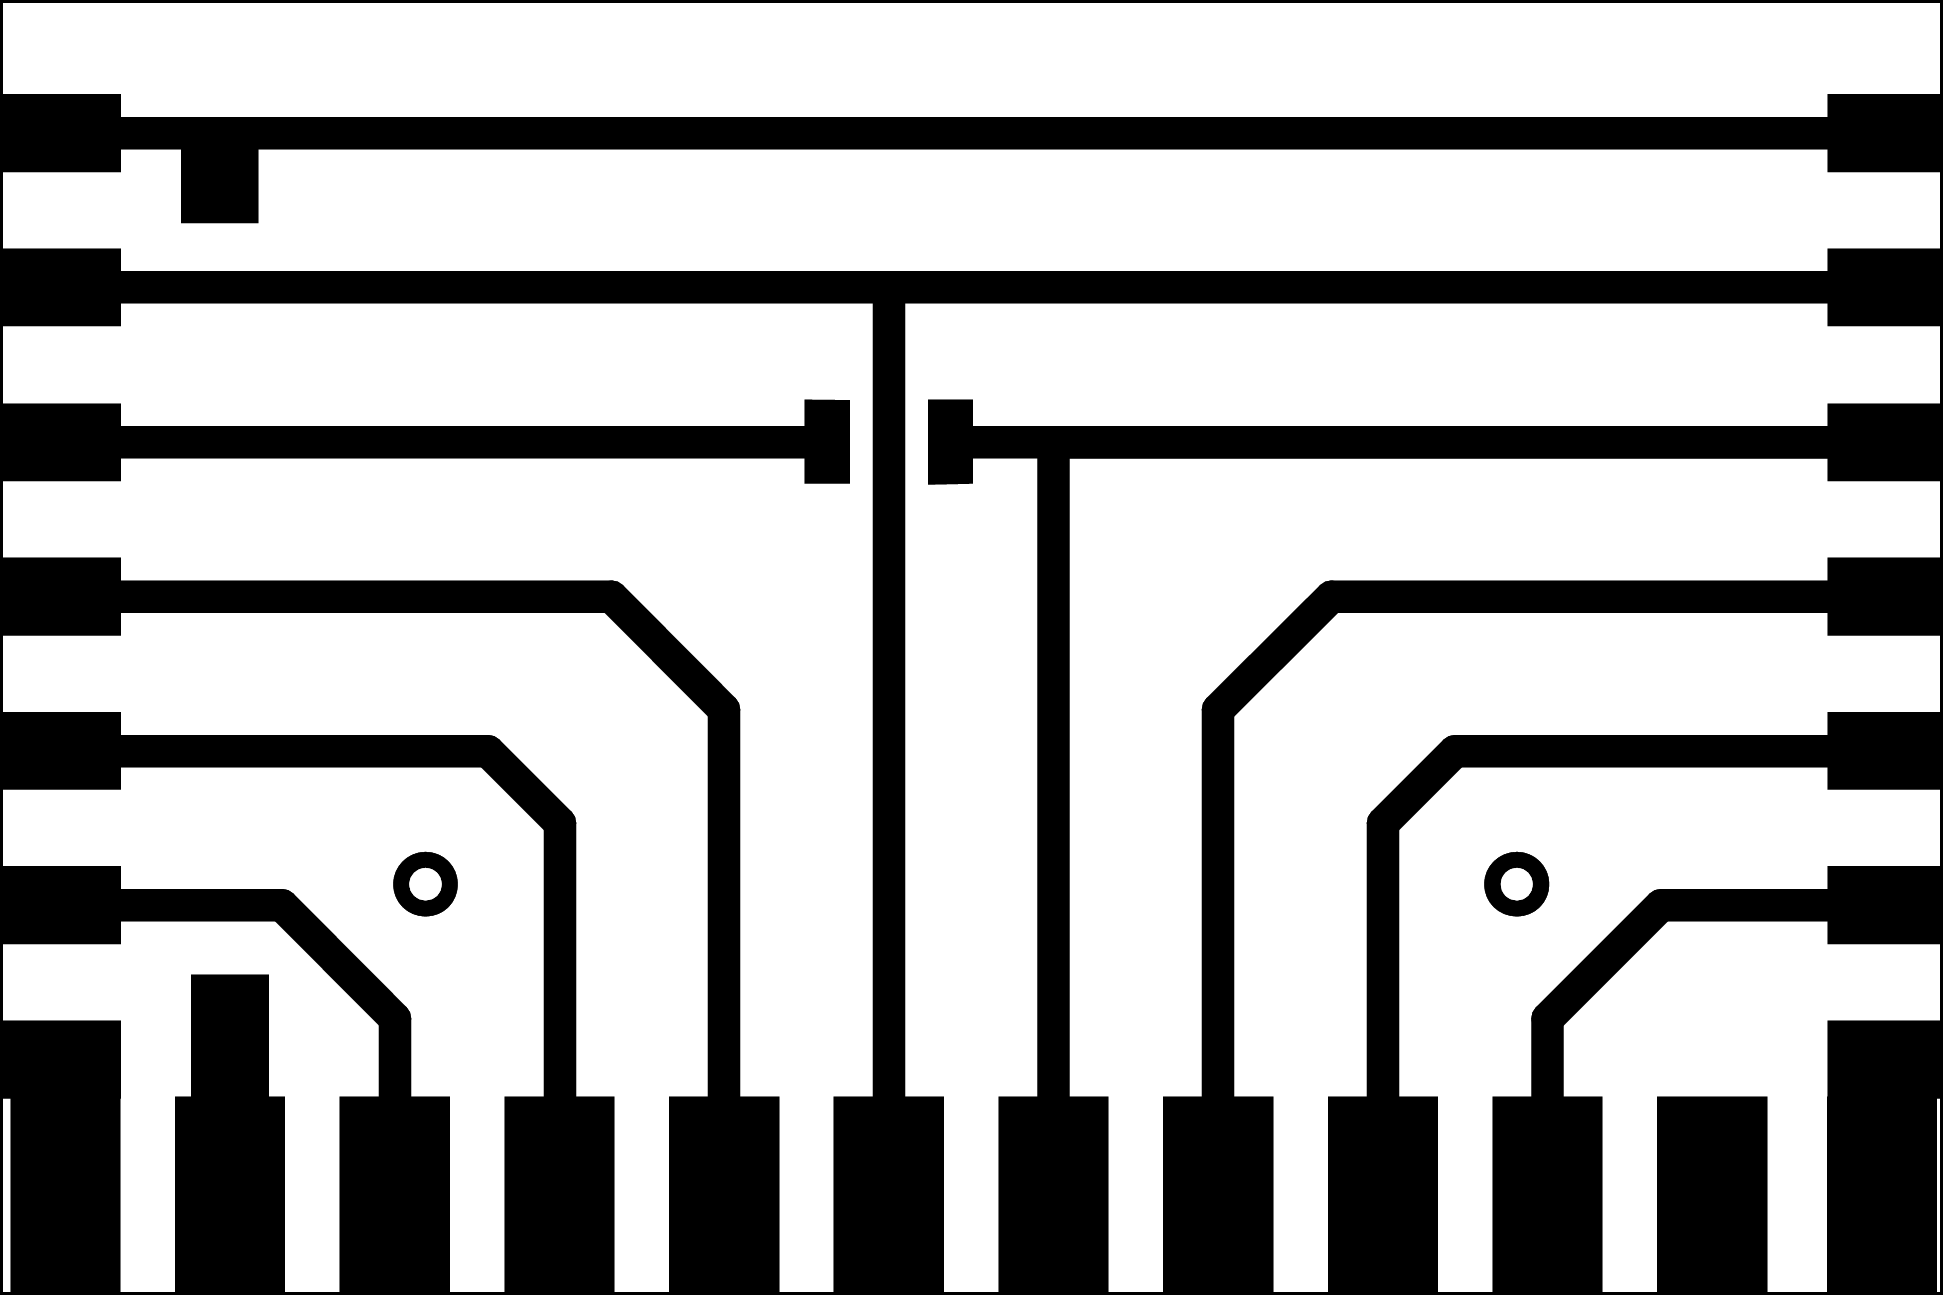
\includegraphics[scale=0.95]{PcbConnector.png}  
	\caption{Печатная плата-соединитель}
	\label{fig:PcbConnector}
\end{figure}

По разработанным рисункам были произведены лазерно-утюжным методом четыре обычных платы и одна плата-соединитель. Затем на них были припаяны компоненты, а сами платы соединены между собой каплями припоя. Вся система была закреплена на деревянной рейке длинной 640 мм с помощью нейлоновых стяжек.

\subsubsection{Тестирование печатной платы. }
Для того, чтобы проверить правильность разработки печатной платы, а также надёжность пайки компонентов, микрофонная решётка была подключена к плате \boardname{} и с помощью заранее разработанной прошивки с каждого микрофона были сняты данные, при воспроизведении звукового сигнала частотой 1 кГц на некотором расстоянии от решётки. Данные были записаны в статическую память, расположенную на плате и переданы на ПК через JTAG отладчик. Затем, с помощью скрипта на языке Python полученные данные были преобразованы в удобную для обработки форму, после чего были обработаны скриптом на языке MATLAB для получения спектра сигнала. Результат такой обработки для одного из микрофонов показан на рисунке~\ref{fig:PdmMicSpectrum}.

\begin{figure}[ht]
	\centering
	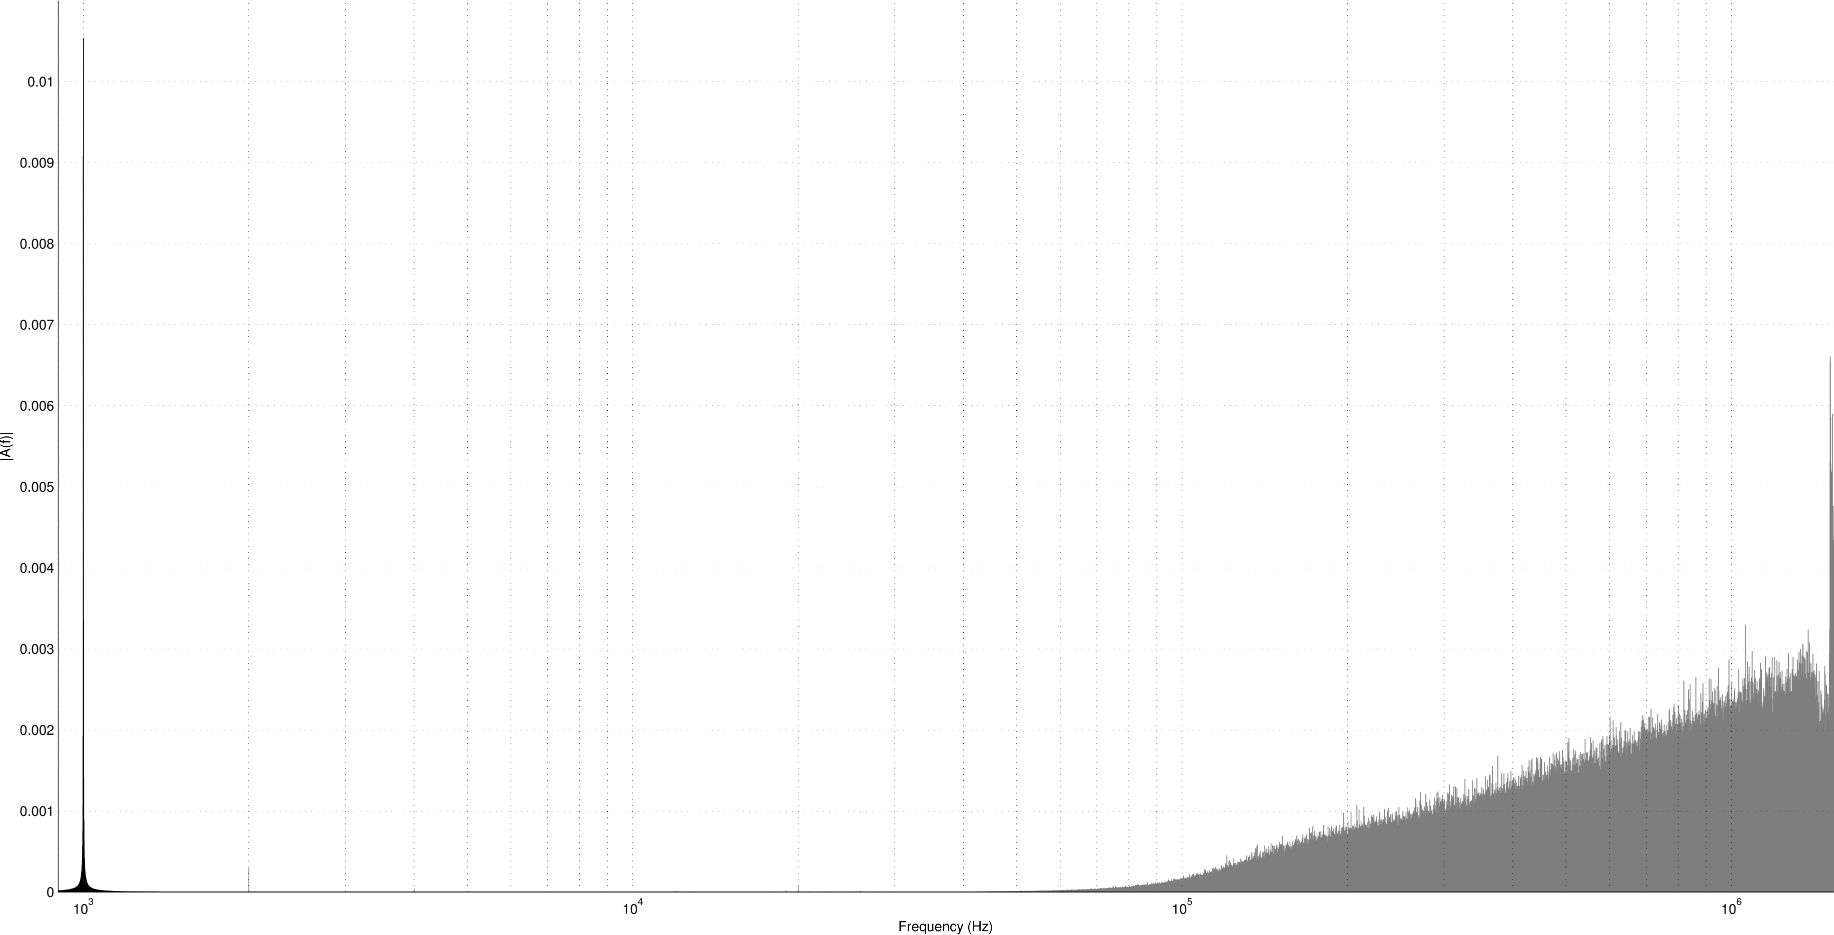
\includegraphics[scale=0.33]{PdmMicSpectrum.png}  
	\caption{Спектр сигнала, полученного с микрофона \micname{}}
	\label{fig:PdmMicSpectrum}
\end{figure}

% **************************************************
\subsection{Разработка многоканального фильтра нижних частот}
\label{section:LowPassFilterBuilding}
 Чтобы снизить стоимость разработки проекта, в качестве датчиков в микрофонной решётке целесообразно применить цифровые PDM-микрофоны. Для того, чтобы произвести дальнейшую обработку сигналов полученных с этих микрофонов, необходимо для начала преобразовать их из формата PDM (см. раздел~\ref{section:pdm}) в формат PCM (импульсно-кодовая модуляция), в котором каждый отсчёт сигнала представлен двоичным числом определённой разрядности. Чтобы понять, как это сделать, необходимо взглянуть на спектр PDM-сигнала, полученного с микрофона \micname{}. Для получения спектра , который изображён на рисунке~\ref{fig:PdmMicSpectrum}. Из рисунка видно, что желаемый сигнал уже является частью спектра исходного сигнала, но помимо него присутствует ещё довольно большое количество шума. Однако, этот шум практически полностью сосредоточен в верхней части спектра. Следовательно, чтобы выделить желаемый сигнал, достаточно всего-лишь пропустить исходный сигнал через фильтр нижних частот (в дальнейшем ФНЧ). Т. к. после фильтрации полученный сигнал больше не будет содержать высокочастотных компонентов, то целесообразно понизить и без того завышенную частоту дискретизации этого сигнала с помощью децимации. Как будет видно в дальнейшем, децимация позволит оптимизировать вычисления производимые фильтром.

\subsubsection{Формулировка требований к ФНЧ. }
Исходя из задачи решаемой проектируемым фильтром, к нему были предъявлены следующие требования:
\begin{itemize}
	\item Способность обеспечивать подавление шума вне полосы пропускания на таком уровне, чтобы данный шум после децимации не сильно ухудшил характеристики полезного сигнала. Чтобы определится со степенью подавления, откроем документацию на микрон \micname. Можно заметить, что отношение сигнал-шум для этого микрофона составляет 61 дБ. Целесообразно выбрать степень подавления таким образом, чтобы с одной стороны не сильно ухудшить этот параметр, а с другой стороны не сделать реализацию фильтра слишком затратной. Поэтому степень подавления была выбрана равной величине в $-100$ дБ.
	\item Для того чтобы не вносить частотные искажения в полезный сигнал, необходимо обеспечить ровную АЧХ во всей полосе пропускания фильтра.
	\item За верхнюю границу полосы пропускания фильтра примем верхнюю границу слышимого человеком диапазона~--- 20~кГц.
	\item Для дальнейшей оптимизации фильтра необходимо выбрать его коэффициент децимации равным степени двойки. Также, согласно теореме Котельникова, этот коэффициент должен снижать первичную частоту дискретизации до уровня как минимум в два раза большего верхней границы фильтра. Исходя из этого выберем коэффициент децимации равным 64.
\end{itemize}

\subsubsection{Выбор типа ФНЧ. }
Согласно разделу~\ref{section:DigitalFilters}, цифровые фильтры бывают двух основных типов: КИХ (раздел~\ref{section:FIR}) и БИХ (раздел~\ref{section:IIR}). Несмотря на некоторые преимущества БИХ фильтров перед КИХ фильтрам, а именно, наличие лучших характеристики при меньшем порядке, а также использование меньшего операций при реализации на цифровых сигнальных процессорах, в данном проекте было решено использовать КИХ-фильтр.

Одной из причин выбора именно КИХ-фильтра является следующий факт. Если взглянуть на структурную схему фильтра (рисунок~\ref{fig:FirStructure}, то можно заметить, что с входным сигналом производится множество операций умножения. А в виду того, что в данном проекте используется FPGA, то целесообразно попытаться избавиться от этой операции, т. к. это позволит освободить дополнительное место на кристалле, занимаемое логикой умножителя. Теперь, вспомним, что мы имеем дело с однобитным сигналом, для которого операция умножения на некую константу $b$ по сути представляет собой взятие этой константы либо со знаком $+$, либо со знаком $-$. Таким образом, полноценный умножитель не потребуется. БИХ-фильтр из-за наличия обратной связи не позволяет выполнить такую оптимизацию.

Абсолютная стабильность и простота реализации также делают КИХ-фильтр очень заманчивым решением.

\subsubsection{Расчет коэффициентов фильтра. }
Для расчётов фильтр была использована утилита FDATool, которая входит в программный пакет MATLAB. Исходя требований к фильтру были рассчитаны его коэффициенты, а затем произведена их квантизация для возможности использования арифметики с фиксированной точкой, при реализации фильтра на FPGA. Результирующий фильтр имеет 18-ти битные коэффициенты, 4095-й порядок и амплитудно-частотную характеристику показанную на рисунке~\ref{fig:LowPassFilterMagnitude}
\begin{figure}[ht]
	\centering
	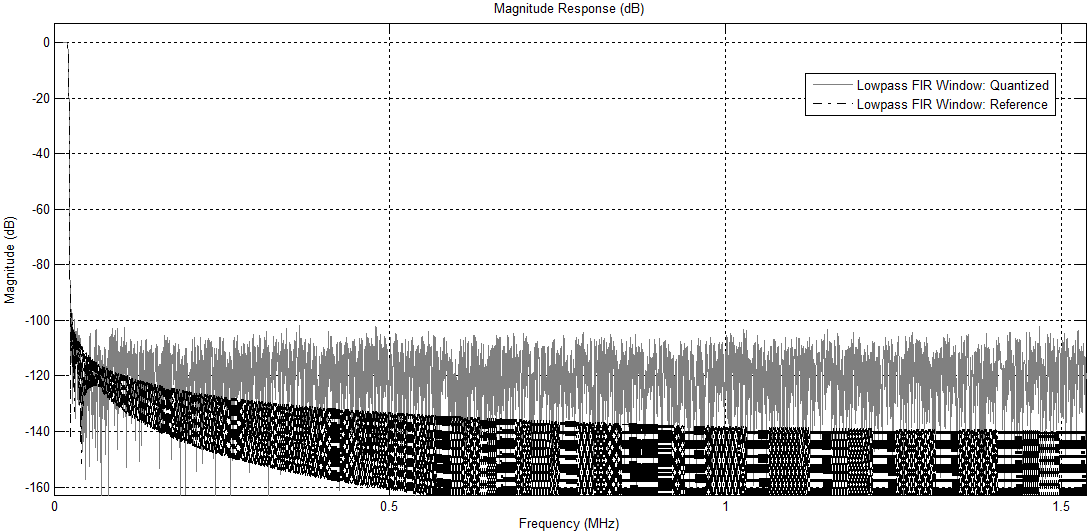
\includegraphics[scale=0.56]{LowPassFilterMagnitude.png}  
	\caption{АЧХ рассчитанного фильтра при использовании коэффициентов с плавающей (серая сплошная линия) и фиксированной (чёрная пунктирная линия) точкой}
	\label{fig:LowPassFilterMagnitude}
\end{figure}

\subsubsection{Реализация фильтра с учётом особенностей FPGA и решаемой фильтром задачи. }
В FPGA серии Cyclone VI фирмы Altera есть встроенный конфигурируемые блоки памяти объёмом 9 килобит каждый. С учётом того, что разрядность коэффициентов фильтра была рассчитана равной 18-ти битам, в каждом блоке поместится 512 коэффициентов. Таким образом, для хранения всех коэффициентов фильтра 4095-го порядка понадобится 8 блоков памяти. Причём, каждый блок можно разместить внутри отдельного вычислительного блока, что обеспечить параллельность вычислений. Структуру каждого вычислительного блока упрощённо так, как показано на рисунке~\ref{fig:LowPassFilterStructure}.
\begin{figure}[ht]
	\centering
	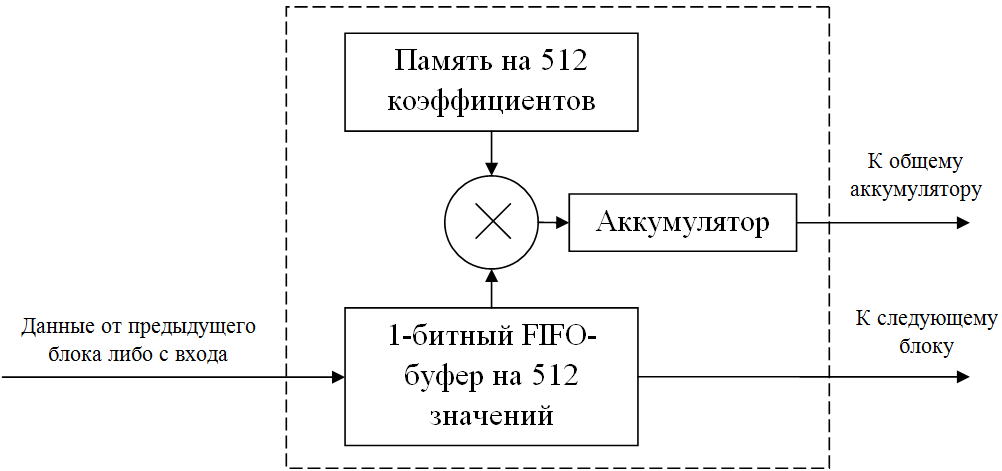
\includegraphics[scale=0.6]{LowPassFilterStructure.png}  
	\caption{Упрощённая структура вычислительного блока КИХ-фильтра, реализованного на FPGA}
	\label{fig:LowPassFilterStructure}
\end{figure}

Микрофон \micname{} тактируется частотой около 3 МГц. Если учесть, что с такой частотой нужно вычислять 512 коэффициентов, то частота каждой операции будет равна 1,5 ГГц. Недорогие ПЛИС не способны работать на такой частоте.
 
Оптимизируем вычисления, имея в виду, что после фильтра производится децимация сигнала с коэффициентом 64. Это означает, что имеет смысл вычислять только каждый 64-й отсчёт. Поэтому, мы можем растянуть во времени вычисление нужных отсчётов, отбросив при этом ненужные. Тогда частота выполнения каждой операции фильтра станет равна всего $3 \cdot{} 512 / 64 = 24$ МГц. Такая частота является вполне приемлемой для используемого в проекте FPGA-чипа.

\subsubsection{Вывод. }
В результате расчётов и анализа возможных оптимизаций, удалось спроектировать фильтр 4095-го порядка, состоящий из восьми вычислительных блоков и работающий на частоте 24 МГц, что всего в 4 раза превосходит частоту дискретизации входного сигнала.

% **************************************************
\subsection{Реализация \dands{} бимформера}
\label{section:BeamformerBuilding}
Согласно разделу~\ref{section:DelayAndSumBeamforming} \dands{} бимформер состоит из сумматора и элементов с контролируемой задержкой. Т. к. реализация сумматора на FPGA является тривиальной, то она не представляет интереса не будет рассмотрена в этой работе.

Рассмотрим способы реализации элемента с контролируемой задержкой.

\subsubsection{Задержка на основе регистров. }
Самым простым решением поставленной задачи является задержка на основе регистров. Её схема показана на рисунке~\ref{fig:RegisterDelay}. Схема состоит из мультиплексора и регистров (или групп регистров в случае многобитного сигнала), соединённых последовательно. Каждый из этих регистров выполняет задержку на один такт. Таким образом, выбрав нужный сигнал с помощью мультиплексора, можно получить сигнал с задержкой на нужное число тактов.
\begin{figure}[ht]
	\centering
	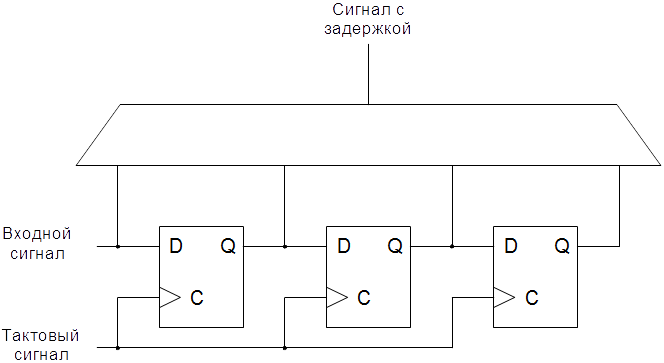
\includegraphics[scale=0.9]{RegisterDelay.png}  
	\caption{Задержка на основе регистров}
	\label{fig:RegisterDelay}
\end{figure}

Данный способ задержки сигнала был опробован при реализации данного проекта. Однако, он оказался не эффективен, т. к. потреблял слишком много ресурсов FPGA-чипа. В результате было решено от него отказаться.

\subsubsection{Задержка на основе блочной памяти. }
Другой подход можно применить при реализации задержки на основе блочной двухпортовой памяти. Такая память показана на рисунке~\ref{fig:MemoryDelay}. Она имеет две шины адреса: А и Б, а также две шины данных: одна для записи, другая для чтения. Входной сигнала поступает на шину А. При этом адрес на шине адреса А меняется на каждом такте. Таким образом, память последовательно заполняется входными данными. При переполнении памяти запись начинается с нулевого адреса, а старые данные стираются. С шины данных Б происходит считывание задержанного сигнала. При этом величина задержки определяется разница адресов А и Б, а её максимальное значение равно ёмкости памяти.

Такой способ организации задержки оказался гораздо экономичнее предыдущего, т. к. при его реализации используются не логические элементы, а блочная память встроенная в FPGA.
\begin{figure}[ht]
	\centering
	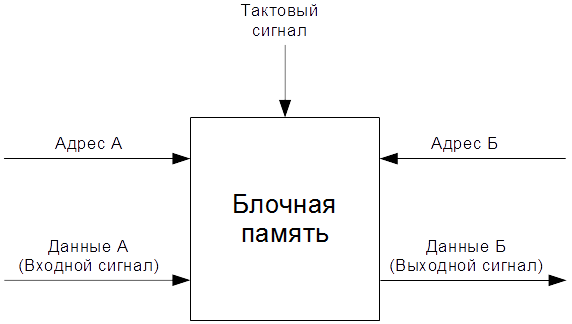
\includegraphics[scale=0.9]{MemoryDelay.png}  
	\caption{Задержка на основе блочной двухпортовой памяти}
	\label{fig:MemoryDelay}
\end{figure}


% **************************************************
\subsection{Разработка полосового фильтра}
\label{section:BandPassFilterBuilding}
Если взглянуть на рисунок~\ref{fig:BeamformerPatterns}, то можно заметить, что \dands{} бимформер имеет плохую пространственную избирательность в области низких частот. А в области высоких частот проявляется эффект пространственного алиасинга, в результате на диаграмме направленности появляются так называемые ложные лепестки (англ. \foreignlanguage{english}{grating lobes}~--- раздражающие лепестки). Чтобы избавится от этих нежелательных эффектов, необходимо чтобы бимформер работал только в определённом диапазоне частот. Для этого понадобится разработать полосовой фильтр.

Зададимся полосой пропускания фильтра 3~--~6 кГц. Степень подавления вне полосы пропускания выберем 80 Дб. Данный фильтр лучше всего реализовать в виде БИХ структуры для экономии ресурсов FPGA. Запустим утилиту FDATool из программного пакета MATLAB и произведём расчёт фильтра согласно исходным данным. Полученный фильтр имеет 32-й порядок и амплитудно-частотную характеристику изображённую на рисунке~\ref{fig:BandPassFilterResponse}.
\begin{figure}[ht]
	\centering
	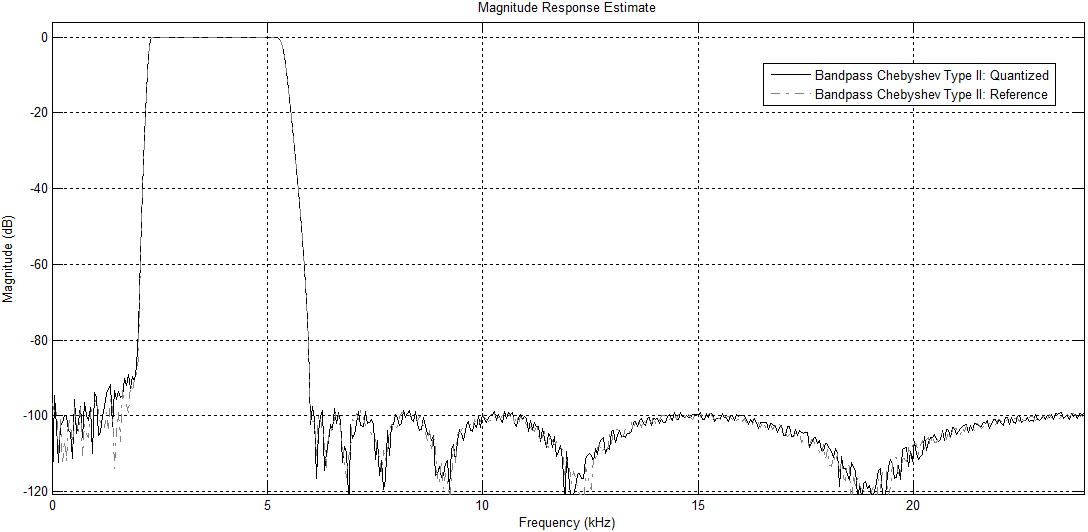
\includegraphics[scale=0.54]{BandPassFilterResponse.png}  
	\caption{Амплитудно-частотная характеристика рассчитанного полосового фильтра при использовании коэффициентов с плавающей (пунктирная серая линия) и фиксированной (чёрная сплошная линия) точкой}
	\label{fig:BandPassFilterResponse}
\end{figure}

В качестве формы БИХ фильтра была выбрана первая прямая форма (англ. \foreignlanguage{english}{Direct Form I Structure}). Такая форма не является самой оптимальной с точки зрения потребляемых ресурсов, однако она позволяет значительно снизить ошибку округления, которая присуща реализации фильтра с использованием арифметики с фиксированной точкой~\cite{Xilinx_IIR}. Также, для снижения ошибки округления и повышения устойчивости фильтра его целесообразно разбить на секции второго порядка (англ. \foreignlanguage{english}{Second Order Section, SOS}). Структура секции второго порядка в первой прямой форме показана на рисунке~\ref{fig:SosStructure}
\begin{figure}[ht]
	\centering
	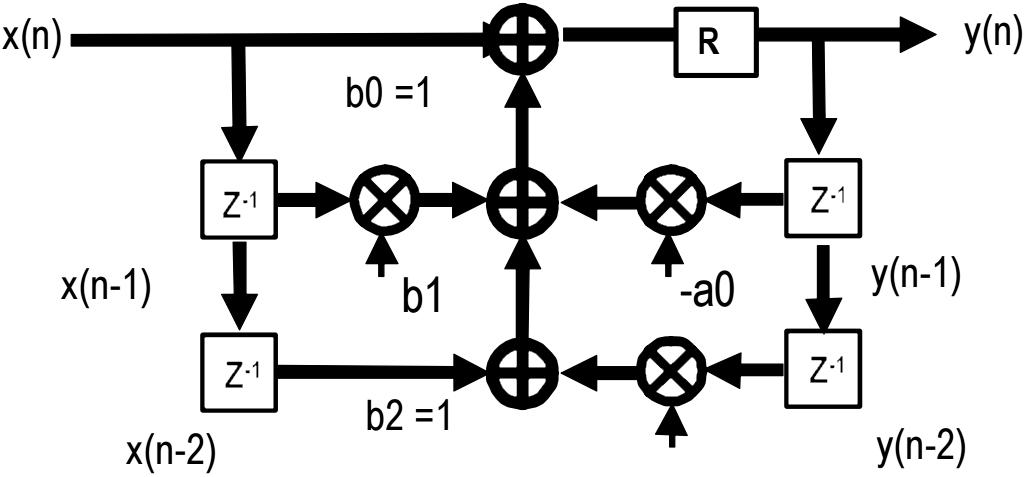
\includegraphics[scale=0.6]{SosStructure.png}  
	\caption{Секция второго порядка в первой прямой форме}
	\label{fig:SosStructure}
\end{figure}

После реализации на языке SystemVerilog данный фильтр был просимулирован в программе ModelSim. Переходная характеристика полученная в результате симуляции полностью совпадает с расчётной. Её вид представлена на рисунке~\ref{fig:BandPassFilterSim}. После, дизайн был скомпилирован и протестирован на плате \boardname{}, а правильность его работы была оценена качественным образом. 
\begin{figure}[ht]
	\centering
	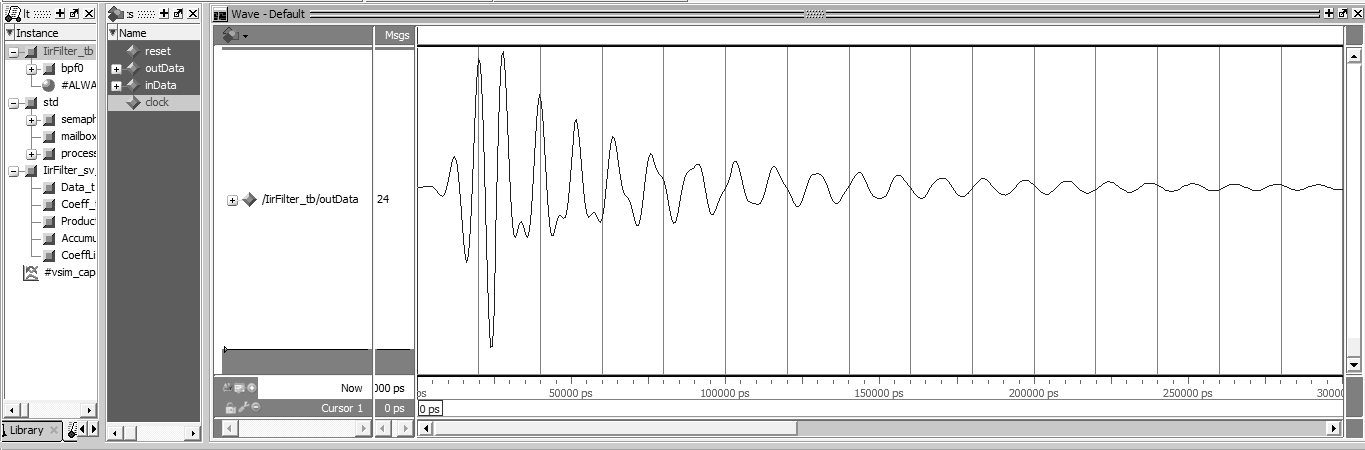
\includegraphics[scale=0.45]{BandPassFilterSim.png}  
	\caption{Переходная характеристика полученная в результате симуляции разработанного фильтра}
	\label{fig:BandPassFilterSim}
\end{figure}

% **************************************************
\subsection{Разработка простейшего видеоадаптера}
\label{section:VideoAdapterBuilding}
В требованиях к проекту указана необходимость отображать результат обработки сигналов на ЖК монитор разрешением 1024 x 768 пикселей. Т. к. на плате \boardname{} присутствуют только VGA-разъём и видео-ЦАП, то для осуществления вывода изображения на монитор придётся формировать сигналы вертикальной и горизонтальной синхронизации средствами FPGA. Также необходимо предусмотреть видео-память для хранения выводимого на дисплей изображения. Рассмотрим подходы к построению данного видеоадаптера.

Самым простым способом реализовать видеоадаптер является организация попиксельного вывода изображения из памяти на дисплей. Подсчитаем объём памяти необходимый для хранения видеоизображения. Яркость свечения каждого пикселя можно записать с помощью одного бита данных (активный и неактивный пиксель). Всего имеется $1024 \cdot{} 768 = 786 432$ пикселей. Таким образом, для хранения целого изображения понадобится 768 кбит. Учитывая, что в выбранном FPGA-чипе встроено 3,89 Мбит памяти, такой дизайн видеоадаптера  занял бы большую часть ресурсов чипа. Следовательно описанный подход не рационален.

\begin{figure}[ht]
	\centering
	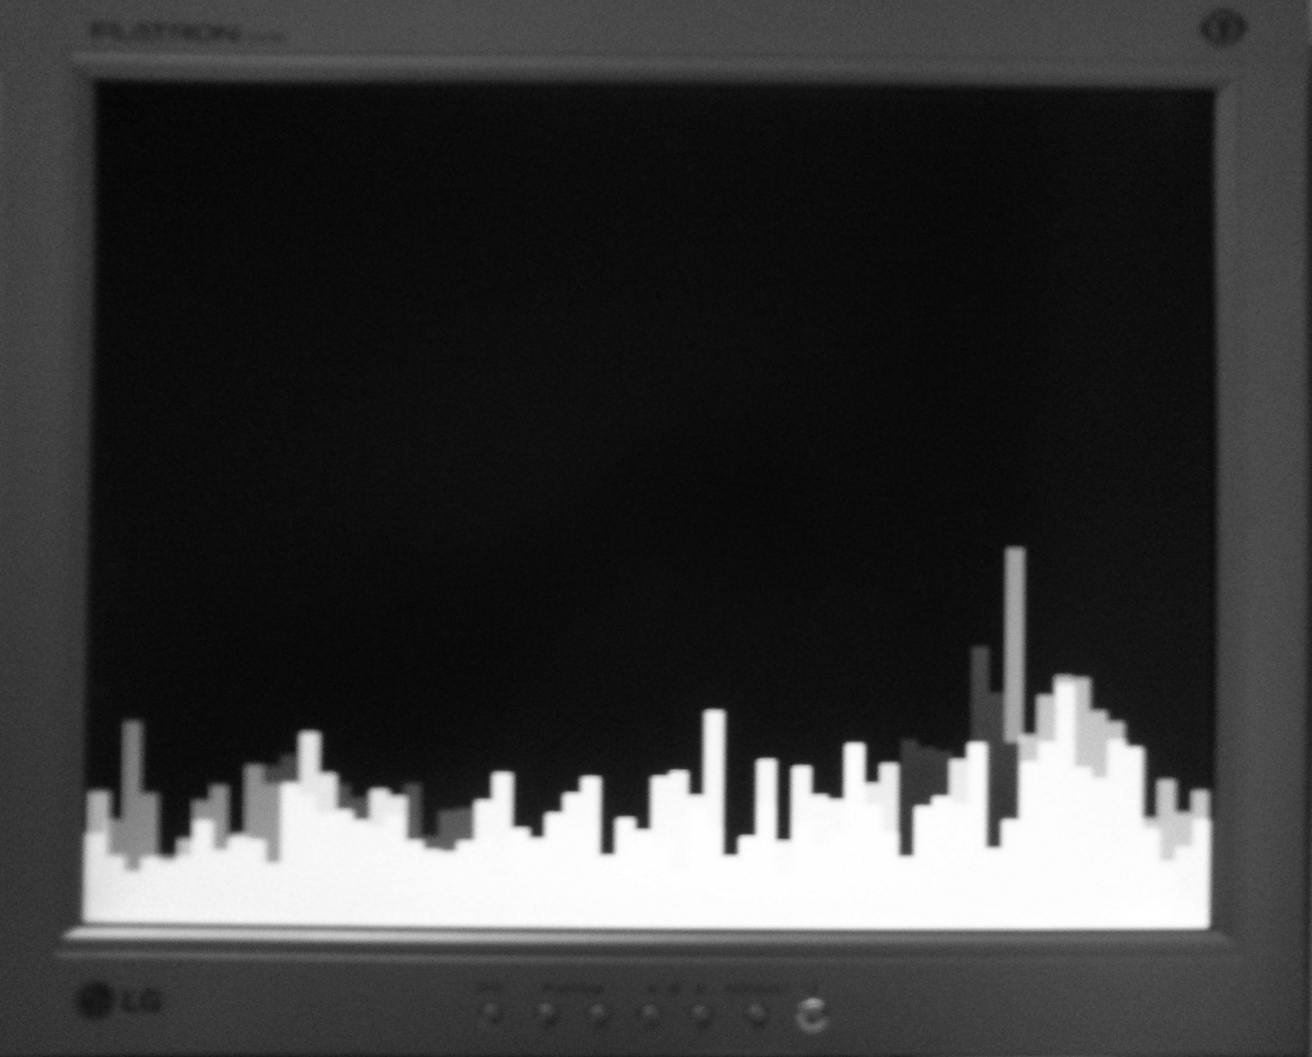
\includegraphics[scale=0.35]{VideoAdapterResult.jpg}  
	\caption{Изображение полученное на ЖК-мониторе с помощью разработанного видеоадаптера}
	\label{fig:VideoAdapterResult}
\end{figure}

Рассмотрим теперь альтернативный подход с учётом особенностей выводимого изображения. В качестве средства для индикации угла с которого пришёл звуковой сигнал определим набор из 64-х столбцов, заполняющих всю ширину экрана. Высота столбца будет будет показывать амплитуду сигнала, а номер столбца~--- угол с которого этот сигнал пришёл (столбец 0~--- $-90^{\circ}$, столбец 63~--- $90^{\circ}$). При этом отпадает необходимость хранить в памяти всё изображение целиком. Цвет пикселя может быть определён исходя из координат этого пикселя и требуемой высоты столбца в зону которого этот пиксель попадает. Таким образом в памяти можно хранить только требуемые высоты столбцов, а её объём определяется исходя из количества градаций высоты столбца и количества столбцов. Для 768-ми градаций и 64-х столбцов этот объем составит всего 7,68 кбит, что ровно на два порядка меньше, чем в предыдущем подходе. В связи с этим именно такое решение было применено в данном проекте.

Результат работы спроектированного видеоадаптера можно увидеть на рисунке~\ref{fig:VideoAdapterResult}.

% **************************************************
\subsection{Результат разработки и решение возникших проблем}
\label{section:ResultAndProblems}
После разработки всех частей и объединения их в единую систему, были произведены испытания полученного устройства. Не смотря на то, что все части по отдельности работали без нареканий, работа устройства в целом оставляла желать лучшего. Главный недостаток заключался в низкой пространственной чувствительности. Т. е. несмотря на отличную чувствительность устройства к звуковым волнам из рабочего диапазона, определить положение источника звука по данным с экрана было хоть и возможно, но несколько затруднительно из-за слабой выраженности направленных свойств микрофонной решётки. Чтобы решить данную проблему было сделано несколько гипотез.

\subsubsection{Калибровка. }
Первая гипотеза состоит в следующем: если один или несколько микрофонов имеют чувствительность намного больше, чем большинство других в системе, то сигнал получаемый с более чувствительных микрофонов будет доминирующим в сумме и из-за всенаправленности отдельного микрофона снизится пространственная чувствительность всей системы.

Чтобы проверить эту гипотезу были произведены измерения чувствительности микрофонов. Для этого была разработана специальная прошивка для платы \boardname{} и написано несколько скриптов на языках TCL, Python и MATLAB, которые позволили записать синал одновременно с 16-ти микрофонов, передать полученные данные на ПК и произвести их анализ. Во время записи на микрофоны был подан звуковой сигнал частотой 100 Гц. Такая частота была выбрана после предварительных экспериментов, показавших, что звуковые волны более высоких частот отражаются от стен помещения и образуют стоячие волны, которые мешают проведению измерений. После записи данных и передачи их на ПК, с помощью пакета MATLAB были построены АЧХ для сигналов с каждого из микрофонов. Результат построения можно увидеть на рисунке~\ref{fig:CalibrationMagnitudeResponse}, из которого видно, что сигналы отличаются незначительно.

\begin{figure}[ht]
	\centering
	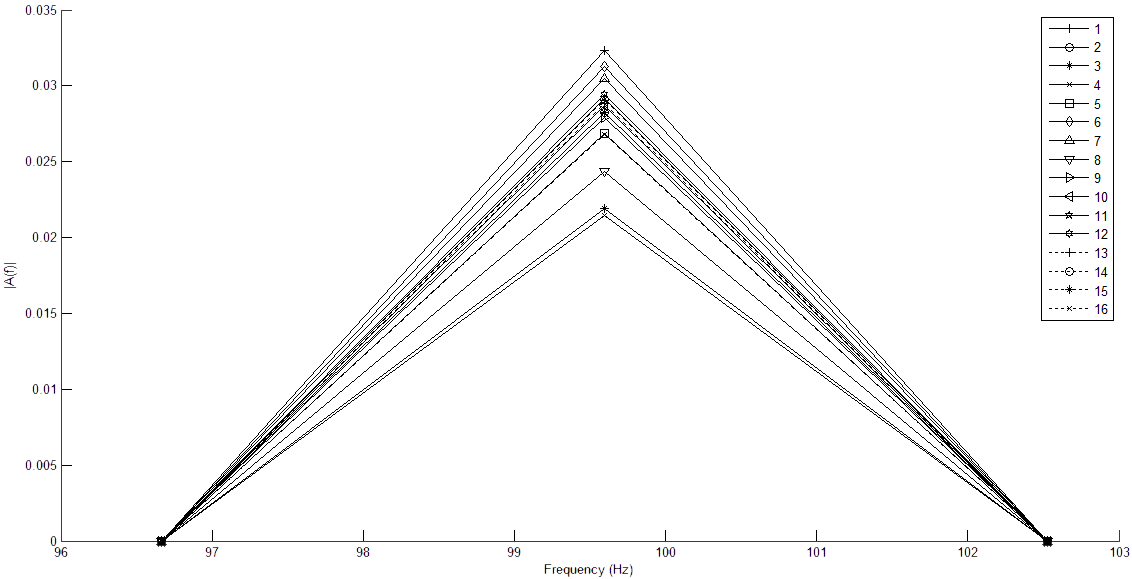
\includegraphics[scale=0.55]{CalibrationMagnitudeResponse.png}  
	\caption{}
	\label{fig:CalibrationMagnitudeResponse}
\end{figure}

Чтобы до конца проверить гипотезу, по данным о чувствительности микрофонов были получены масштабирующие коэффициенты, а в систему добавлен новый элемент~--- калибратор, который производит ослабление сигналов с микрофонов в соответствии с этими коэффициентами. После введения в систему калибратора, были снова проведены тесты пространственной чувствительности. Однако, каких либо заметных улучшений не наблюдалось и данная гипотеза была отвергнута.

\subsubsection{Фазировка. }
Другая выдвинутая гипотеза строится на предположении о том, что микрофоны могут быть не сфазированы из-за особенностей их производства. Работая в противофазе такие микрофоны выдавали бы сигналы не способные коррелировать, что могло бы обуславливать низкую пространственную чувствительность системы.

Для проверки данной гипотезы были взяты данные, полученные в процессе калибровки и по ним построены фазовые характеристики сигналов. Результат этого построения представлен на рисунке~\ref{fig:CalibrationPhaseResponse}. Из этих характеристик видно, что сдвига фаз в $180^{\circ}$ между сигналами не наблюдается. Таким образом, данная гипотеза была также отвергнута.

\begin{figure}[ht]
	\centering
	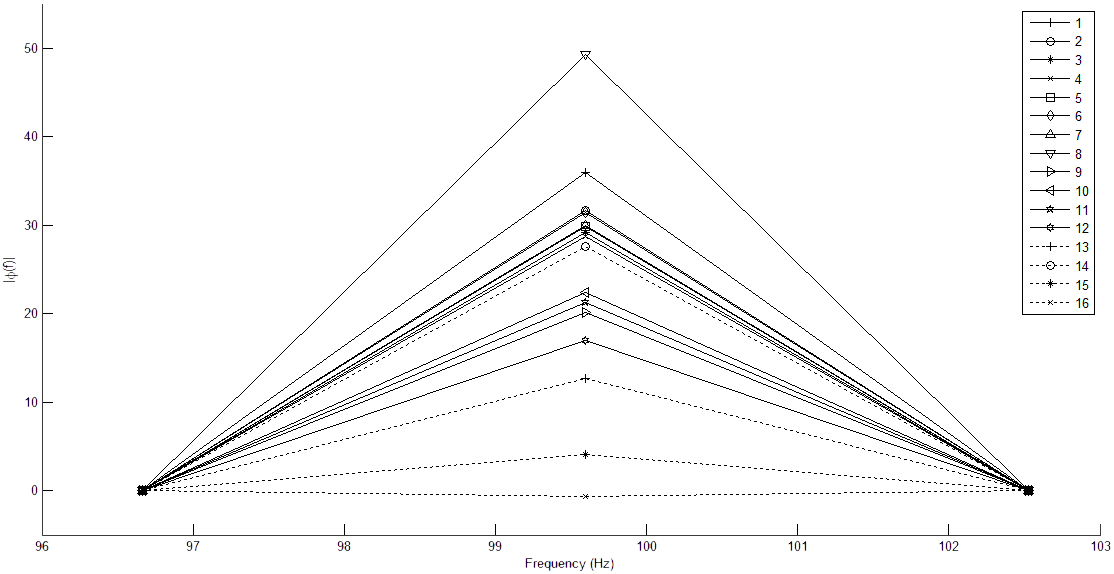
\includegraphics[scale=0.55]{CalibrationPhaseResponse.png}  
	\caption{}
	\label{fig:CalibrationPhaseResponse}
\end{figure}

\subsubsection{Случайные сдвиги фаз. }
На основе данных полученных при проверке предыдущей гипотезы, возникла третья гипотеза. Если взглянуть ещё раз на рисунок~\ref{fig:CalibrationPhaseResponse}, то можно заметить наличие случайных сдвигов фаз между сигналами хоть и меньших $180^{\circ}$, но всё же значительных и потенциально способных привести к наблюдаемым негативным эффектам. Причина этих сдвигов на данный момент не ясна, и может заключаться в неправильно выполненных измерениях. Тогда данную гипотезу также придётся отвергнуть.

Чтобы проверить эту гипотезу, необходимо вычислить задержки вносимые внутренними узлами микрофона по полученным фазовым сдвигам и попытаться их компенсировать. Однако это выходит за рамки данного дипломного проекта по причине ограниченного времени.